This panel is provided for the user to specify multiple existing SimCenter
event files.  If more than one event is specified it is done to
provide the UQ engine with a discrete set of events to choose
from\textemdash it is not done with the intention of specifying that
one event follows another.  The panel presented initially to the user
is as shown in \Cref{fig:figure4}.

\begin{figure}[!htbp]
  \centering {
    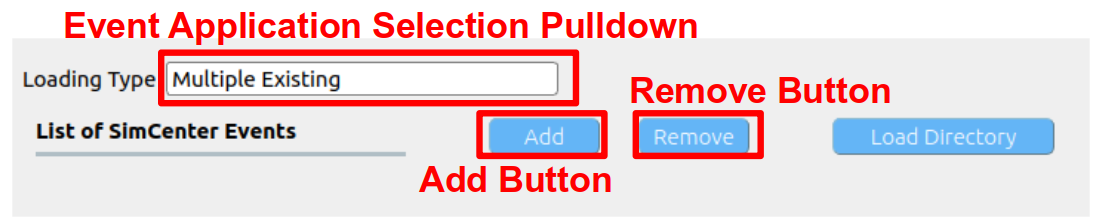
\includegraphics[width=0.8\textwidth]
    {usage/figures/multipleExisting1.png} }
  \caption{\texttt{Multiple Existing} events selected as EVT loading type}
  \label{fig:figure4}
\end{figure}

To add a new event, the user presses the \texttt{Add} button. This adds an
event to the panel. Pressing the button multiple times will keep
adding events to the panel. \Cref{fig:figure5} shows the state after
the button has been pressed twice, and data entered for the ElCentro
and Rinaldi Events.

\begin{figure}[!htbp]
  \centering {
    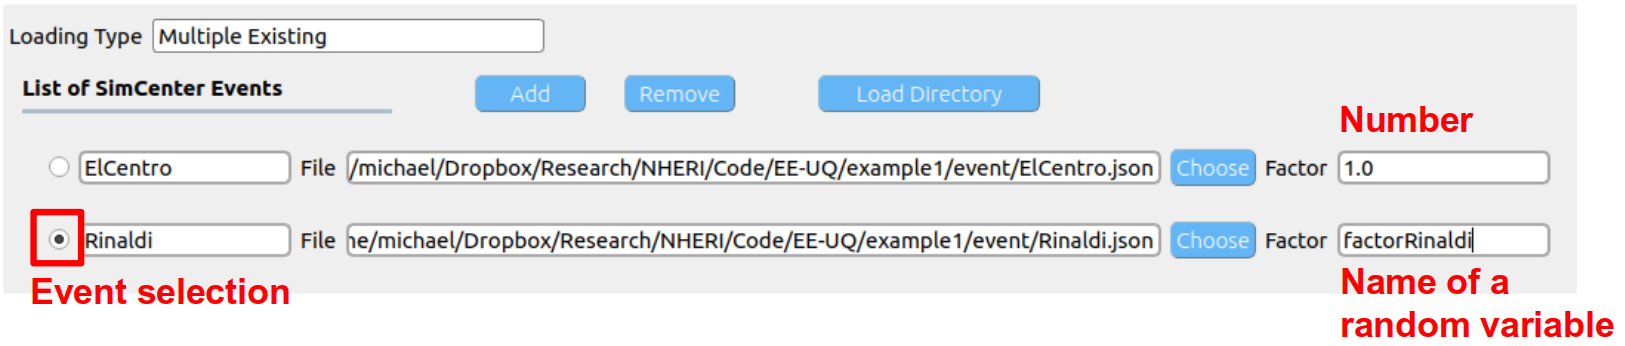
\includegraphics[width=0.8\textwidth]
    {usage/figures/multipleExisting2.png} }
  \caption{Adding new event under \texttt{Multiple Existing} loading type}
  \label{fig:figure5}
\end{figure}

The user can enter the full path manually to the file or use the
\texttt{Choose} button, which brings up your typical file search screen.  By
default, a scaling factor of 1.0 is assigned to the event.  The user
can change this to another real value (AT PRESENT DO NOT USE INTEGER)
or the user has the option of defining this to be a random variable by
entering a name as shown for the second event.

Note that this variable name must not start with a number, or contain
any spaces or special characters, i.e. no -, +,..

The \texttt{Remove} button is pressed to remove events. To remove an
event, the user must first select which events they wish to remove,
done by clicking in the small circle at the start of the event. Once
the events to remove have been selected, the user removes all these
selected evens by pressing the \texttt{Remove} button.

If the user has multiple events to load, all the event files may first
be placed by the user into a separate folder. If the user presses the
\texttt{Load Directory} button, the user will be able to choose a directory and the
application will load all the event files (any file with a \texttt{.json}
suffix) into the widget by choosing the directory. Initially, each
event will be given a load factor of 1.0.  Should the user include in
that directory a file named \texttt{Records.txt}, the application will open that
file and load the events and assigned load factors from that
file. Each line in \texttt{Records.txt} is considered to represent a record, and
contains 2 comma separated values: the first value being the event
file and the second value the event factor. An example \texttt{Records.txt} is
as shown below:

\begin{verbatim}
ElCentro.json,1.5
Rinaldi.json,2.0
\end{verbatim}

Random Variables: The user can, as mentioned, enter a string in the
factor field to specify that the factor is to be considered a random
variable. Subsequently in the UQ panel the user must provide
information on the random variables distribution. Also, if multiple
events are specified, the event itself will be treated as a random
variable, with each event being part of the discrete set of possible
events.
